\section{Python Problem - Wiener's LMS}\label{sec:p5}

\begin{enumerate}[(a)]
\item Figure \ref{fig:p5a} illustrates the prediction problem as an adaptive filter diagram, where the input is $x[n]$, the reference $d[n] = x[n+1] = \alpha x[n] + s[n] - 0.5 s[n-1]$, and the cost function $C(w) = \Expect{\abs{e[n]}^2} = \Expect{\abs{d[n] - y[n]}^2} = \Expect{\abs{d[n] - w^\top X[n]}^2}$.
\begin{figure}[htbp]
	\centering
	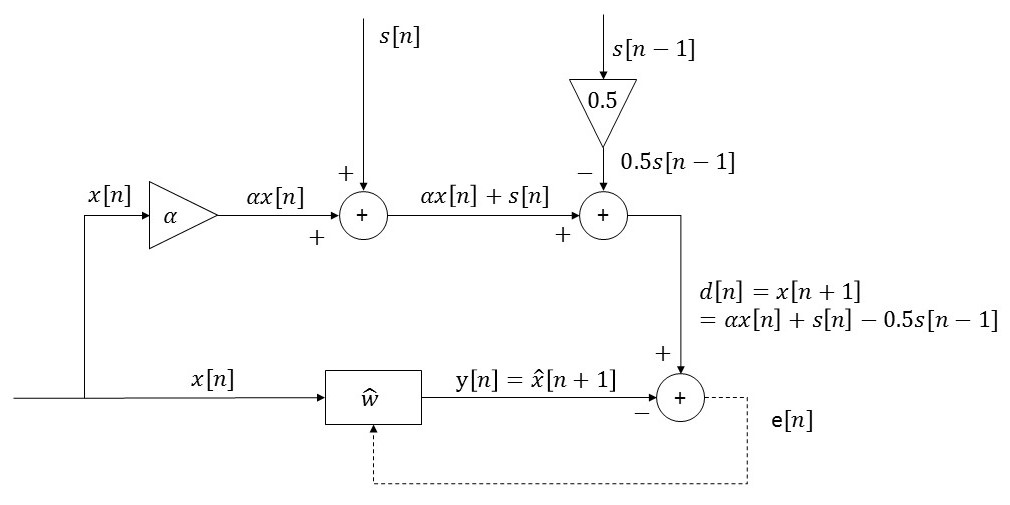
\includegraphics[width=\textwidth]{images/p5a}
	\caption{Adaptive filter diagram}
	\label{fig:p5a}
\end{figure}

\item 
We have \[x[n+1] = \alpha x[n] + s[n] - 0.5 s[n-1]\] Therefore, its Z-transform is
\begin{align*}
	X(z)z &= \alpha X(z) + S(z) -0.5 S(z) z^{-1} \\
	\Leftrightarrow X(z)(z-\alpha) &= S(z) \frac{1 - 0.5 z^{-1}}{z - \alpha} \\
	\Rightarrow H(z) &= \frac{1 - 0.5 z^{-1}}{z - \alpha}
\end{align*}
Since $A_s(z) = 1$,
\begin{align*}
	A_x(z)
	&= H(z)H(z^{-1}) \\
	&= \frac{1 - 0.5 z^{-1}}{z - \alpha} \frac{1 - 0.5 z}{z^{-1} - \alpha} \\
	&= (1.25 - 0.5z - 0.5z^{-1})\frac{1}{1 - \alpha z + \alpha z^{-1} - \alpha^2}\\
	&= (1.25 - 0.5z - 0.5z^{-1})\frac{1}{1 - \alpha z}\frac{1}{1 - \alpha z^{-1}}
\end{align*}
Let $P(z) = 1.25 - 0.5z - 0.5z^{-1}$ and $G(z) = \frac{1}{1 - \alpha z}\frac{1}{1 - \alpha z^{-1}}$. We notice that, by geometric series
\[\frac{1}{1 - \alpha z} = \sum_{m=0}^{\infty}(\alpha z)^n\]
\[\frac{1}{1 - \alpha z^{-1}} = \sum_{m=0}^{\infty}\alpha^m z^{-m}\]
Therefore
\[G(z) = \sum_{m \geq 0, n \geq 0} \alpha^{n+m} z^{n-m}\]

Let $g[\cdot]$ be the inverse z-transform of $G(z)$. We see that $g[0]$ is the sum subject to $n - m = 0 \Leftrightarrow n = m$, i.e.
\[g[0] = \sum_{m \geq 0} \alpha^{n+m} = \sum_{m \geq 0} \alpha^{2m}\]
In general
\[g[k] = \sum_{m \geq 0} \alpha^{2m+k} = \alpha^k \sum_{m=0}^{\infty} \alpha^{2m} = \frac{\alpha^k}{1- \alpha^2}\]
Therefore
\[	a_x[k] = \frac{1}{1- \alpha^2} (1.25 \alpha^{k} - 0.5 \alpha^{k+1} - 0.5 \alpha^{k-1}) \]

\item Figure \ref{fig:p5-1}-\ref{fig:p5-6} show the results of different approaches with varied choices of $\alpha$ and $L$. Overall, the probabilistic result is closer to LMS than statistical one. When $\alpha = 0$, statistical and LMS approaches have higher error than when $\alpha = 0.9$. Moreover, larger $L$ also reduces the prediction error.
\begin{figure}[htbp]
	\centering
	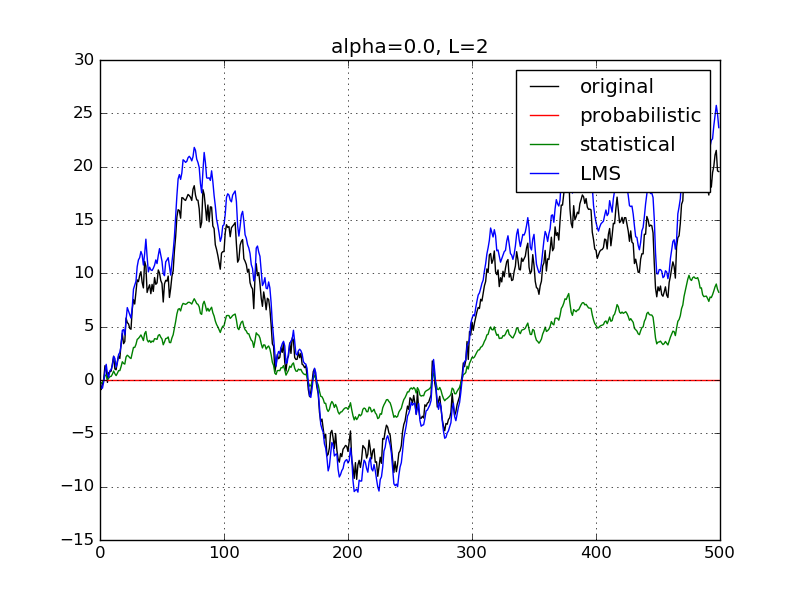
\includegraphics[width=\textwidth]{images/p5-1}
	\caption{$\alpha=0, L=2$.}
	\label{fig:p5-1}
\end{figure}

\begin{figure}[htbp]
	\centering
	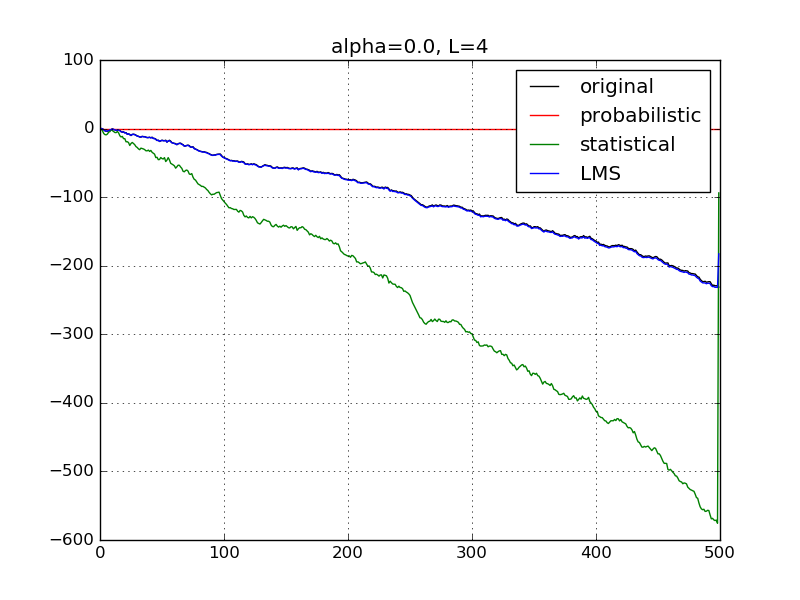
\includegraphics[width=\textwidth]{images/p5-2}
	\caption{$\alpha=0, L=4$.}
	\label{fig:p5-2}
\end{figure}

\begin{figure}[htbp]
	\centering
	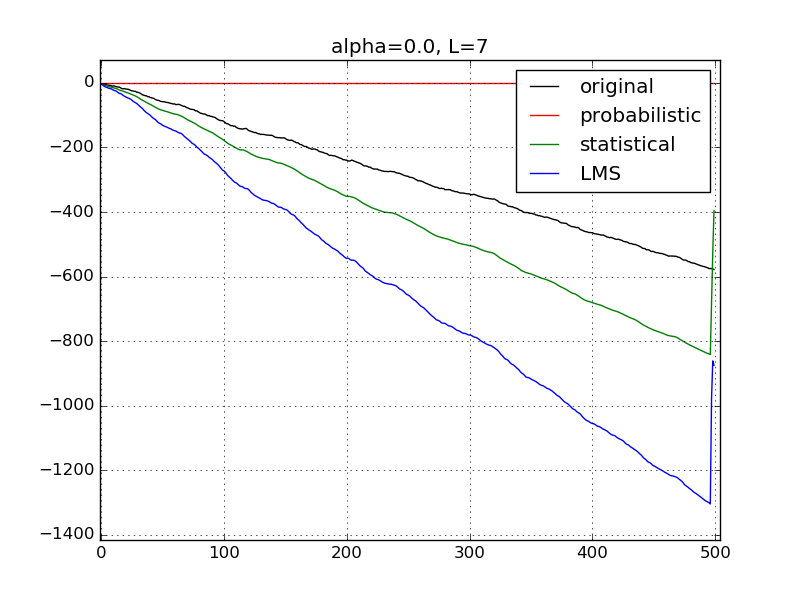
\includegraphics[width=\textwidth]{images/p5-3}
	\caption{$\alpha=0, L=7$.}
	\label{fig:p5-3}
\end{figure}

\begin{figure}[htbp]
	\centering
	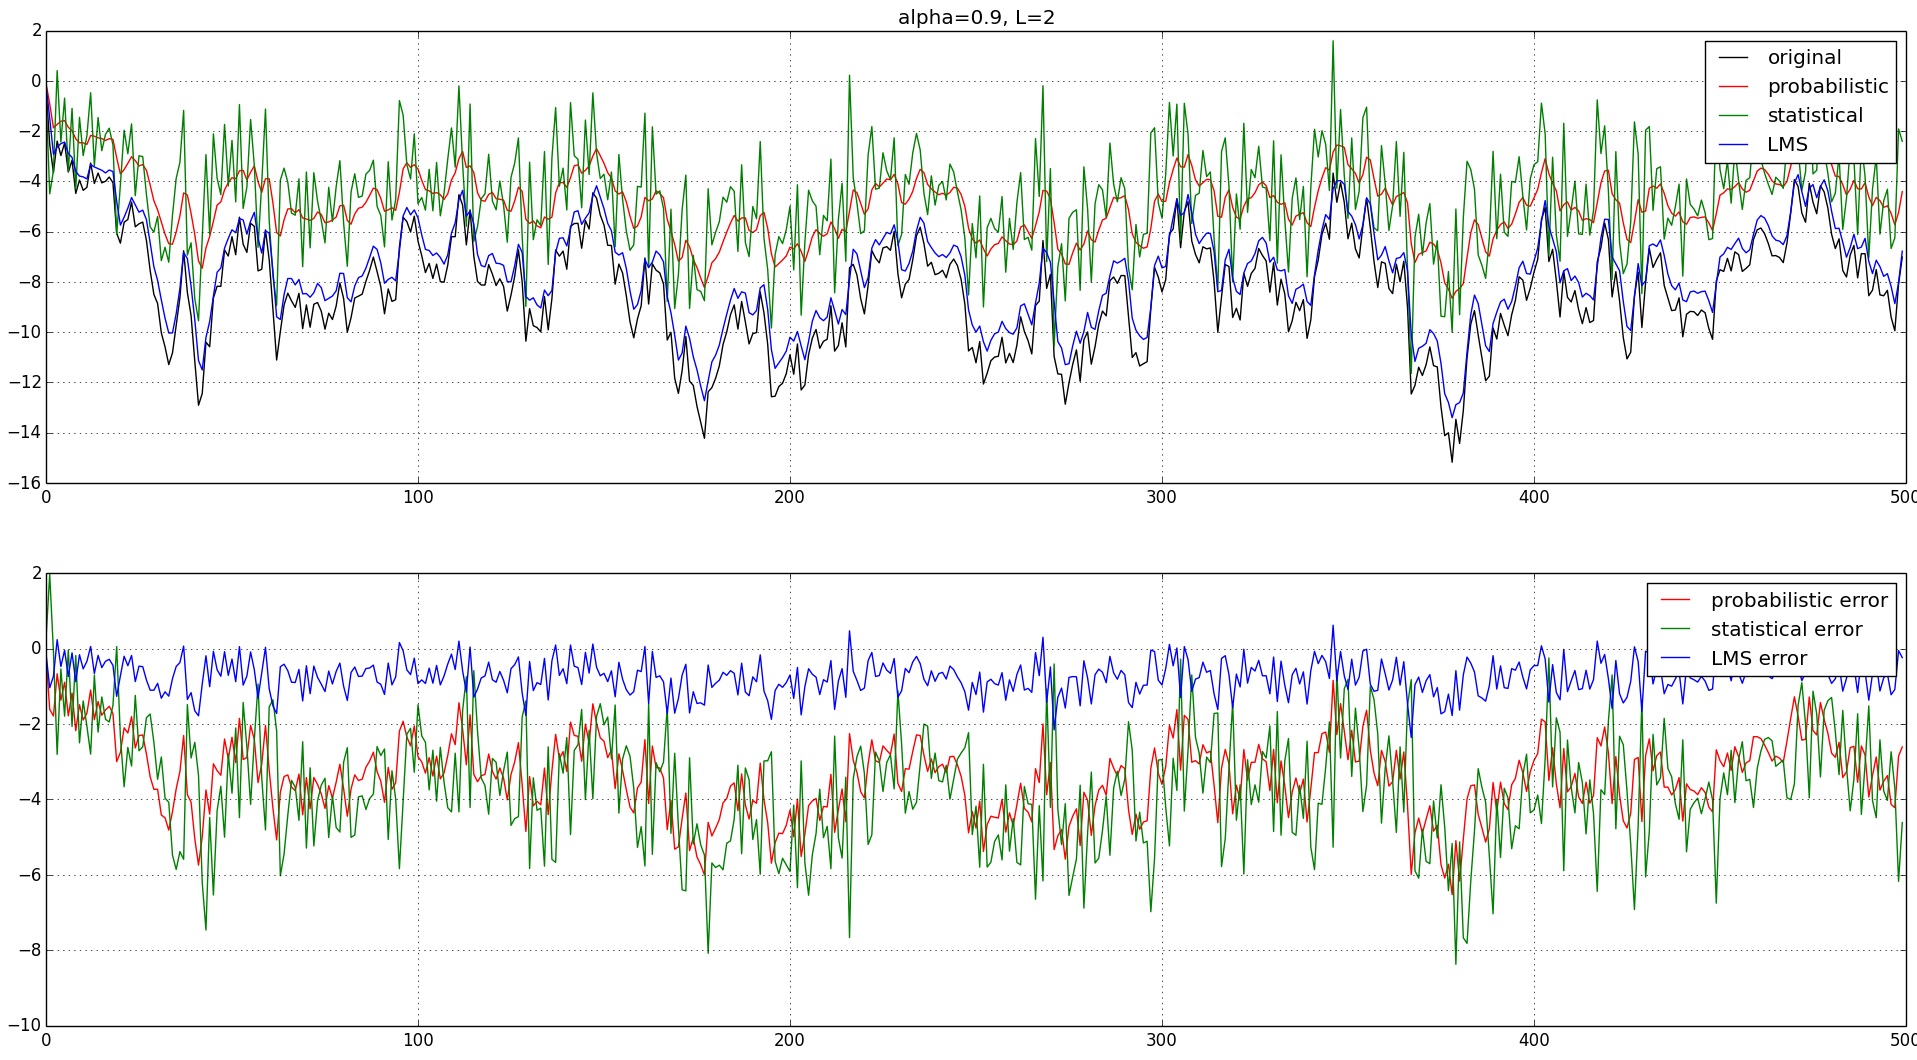
\includegraphics[width=\textwidth]{images/p5-4}
	\caption{$\alpha=0.9, L=2$.}
	\label{fig:p5-4}
\end{figure}

\begin{figure}[htbp]
	\centering
	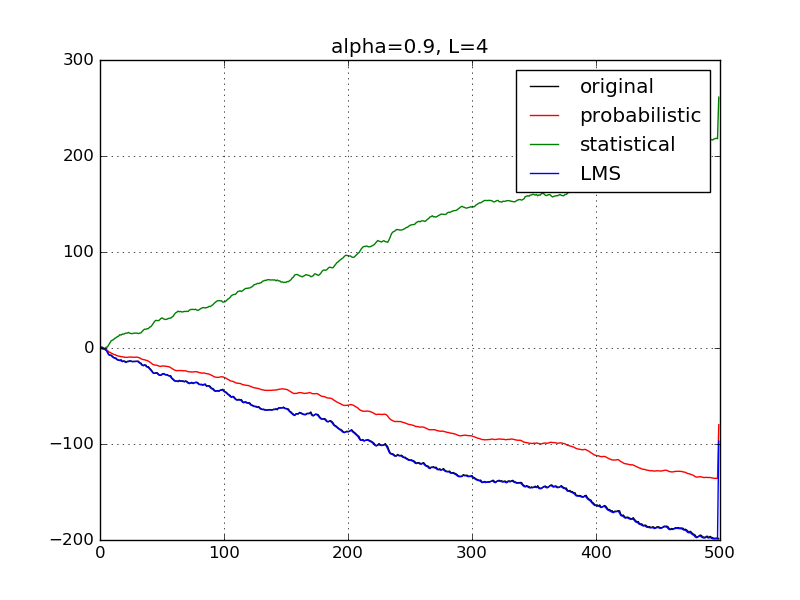
\includegraphics[width=\textwidth]{images/p5-5}
	\caption{$\alpha=0.9, L=4$.}
	\label{fig:p5-5}
\end{figure}

\begin{figure}[htbp]
	\centering
	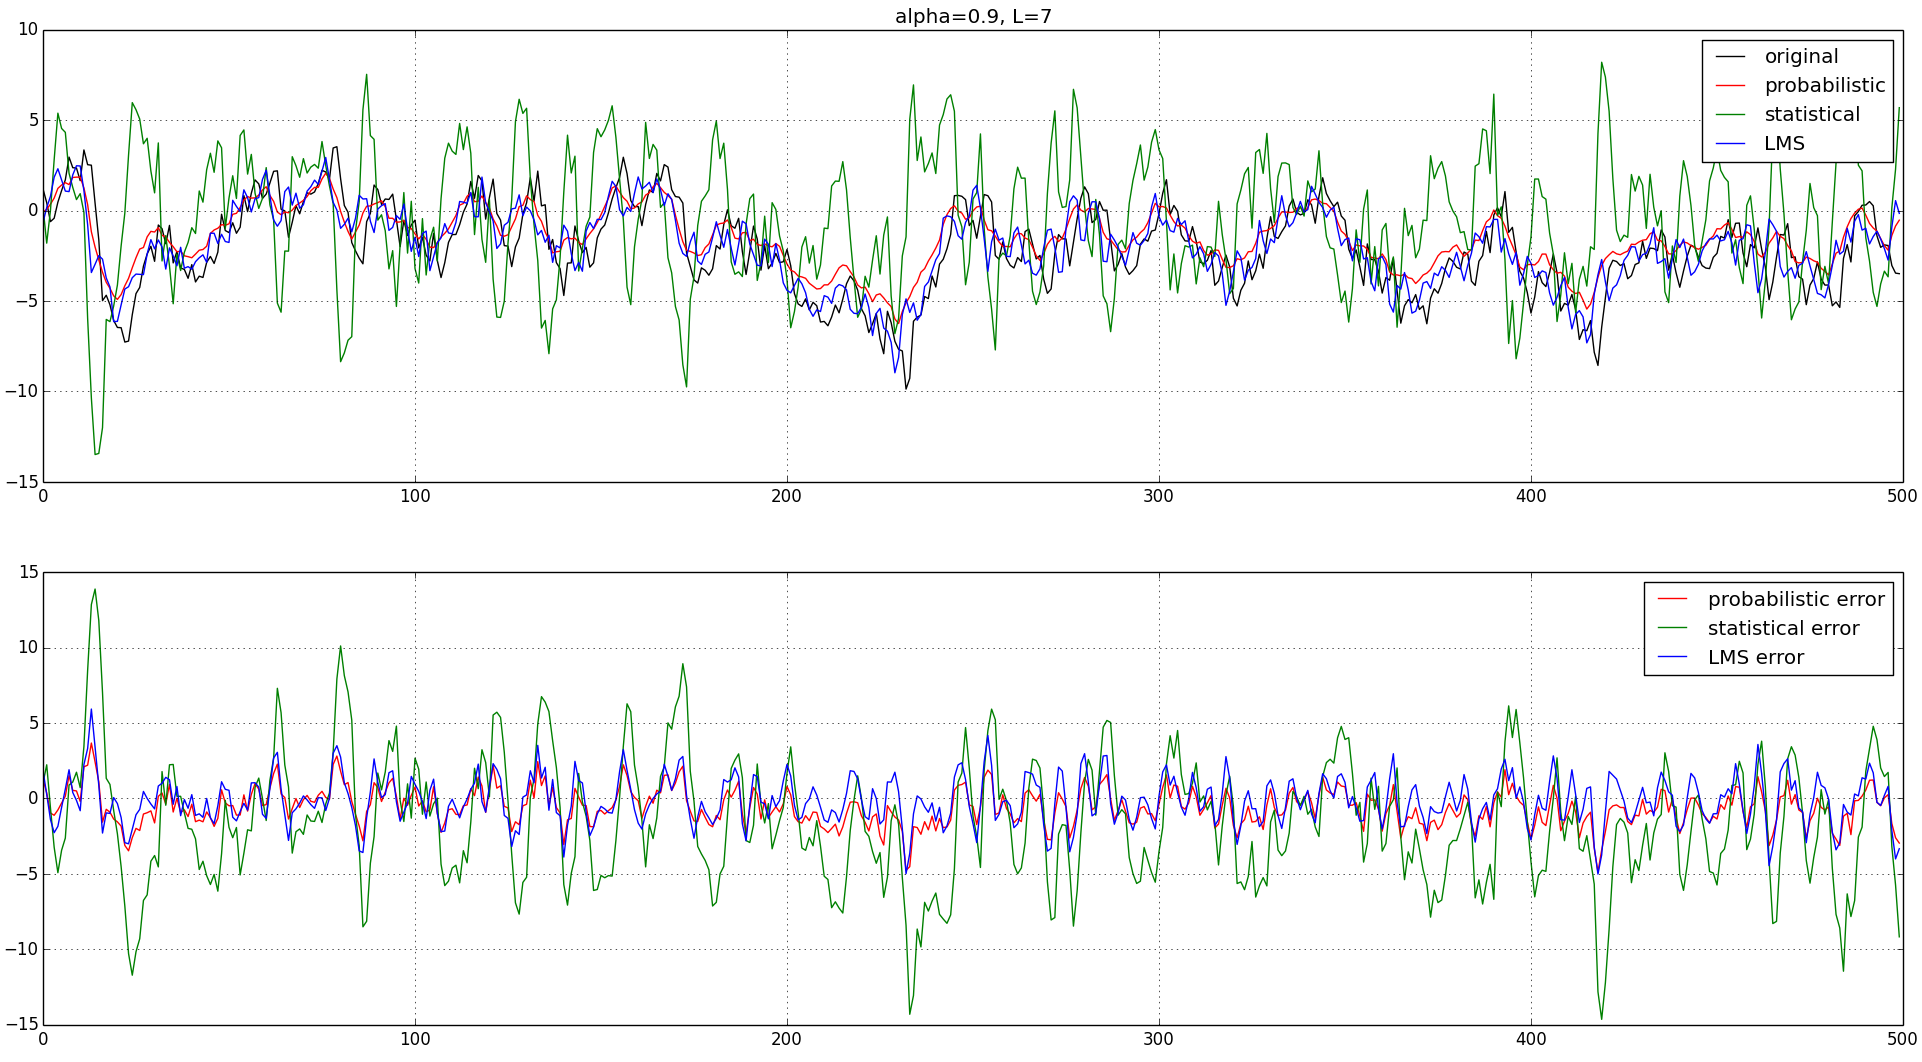
\includegraphics[width=\textwidth]{images/p5-6}
	\caption{$\alpha=0.9, L=7$.}
	\label{fig:p5-6}
\end{figure}

\end{enumerate}

\newpage